\documentclass[18pt]{article}
\usepackage[utf8]{inputenc}
\usepackage[T1]{fontenc}
\usepackage{ragged2e}
\usepackage{caladea}
\usepackage{graphicx}
\usepackage{longtable}
\usepackage{wrapfig}
\usepackage{rotating}
\usepackage{epigraph}
\usepackage[normalem]{ulem}
\usepackage{hyperref}
\usepackage{amsmath}
\usepackage{amssymb}
\usepackage{capt-of}
\usepackage{hyperref}
\usepackage{fancyhdr}

\title{
 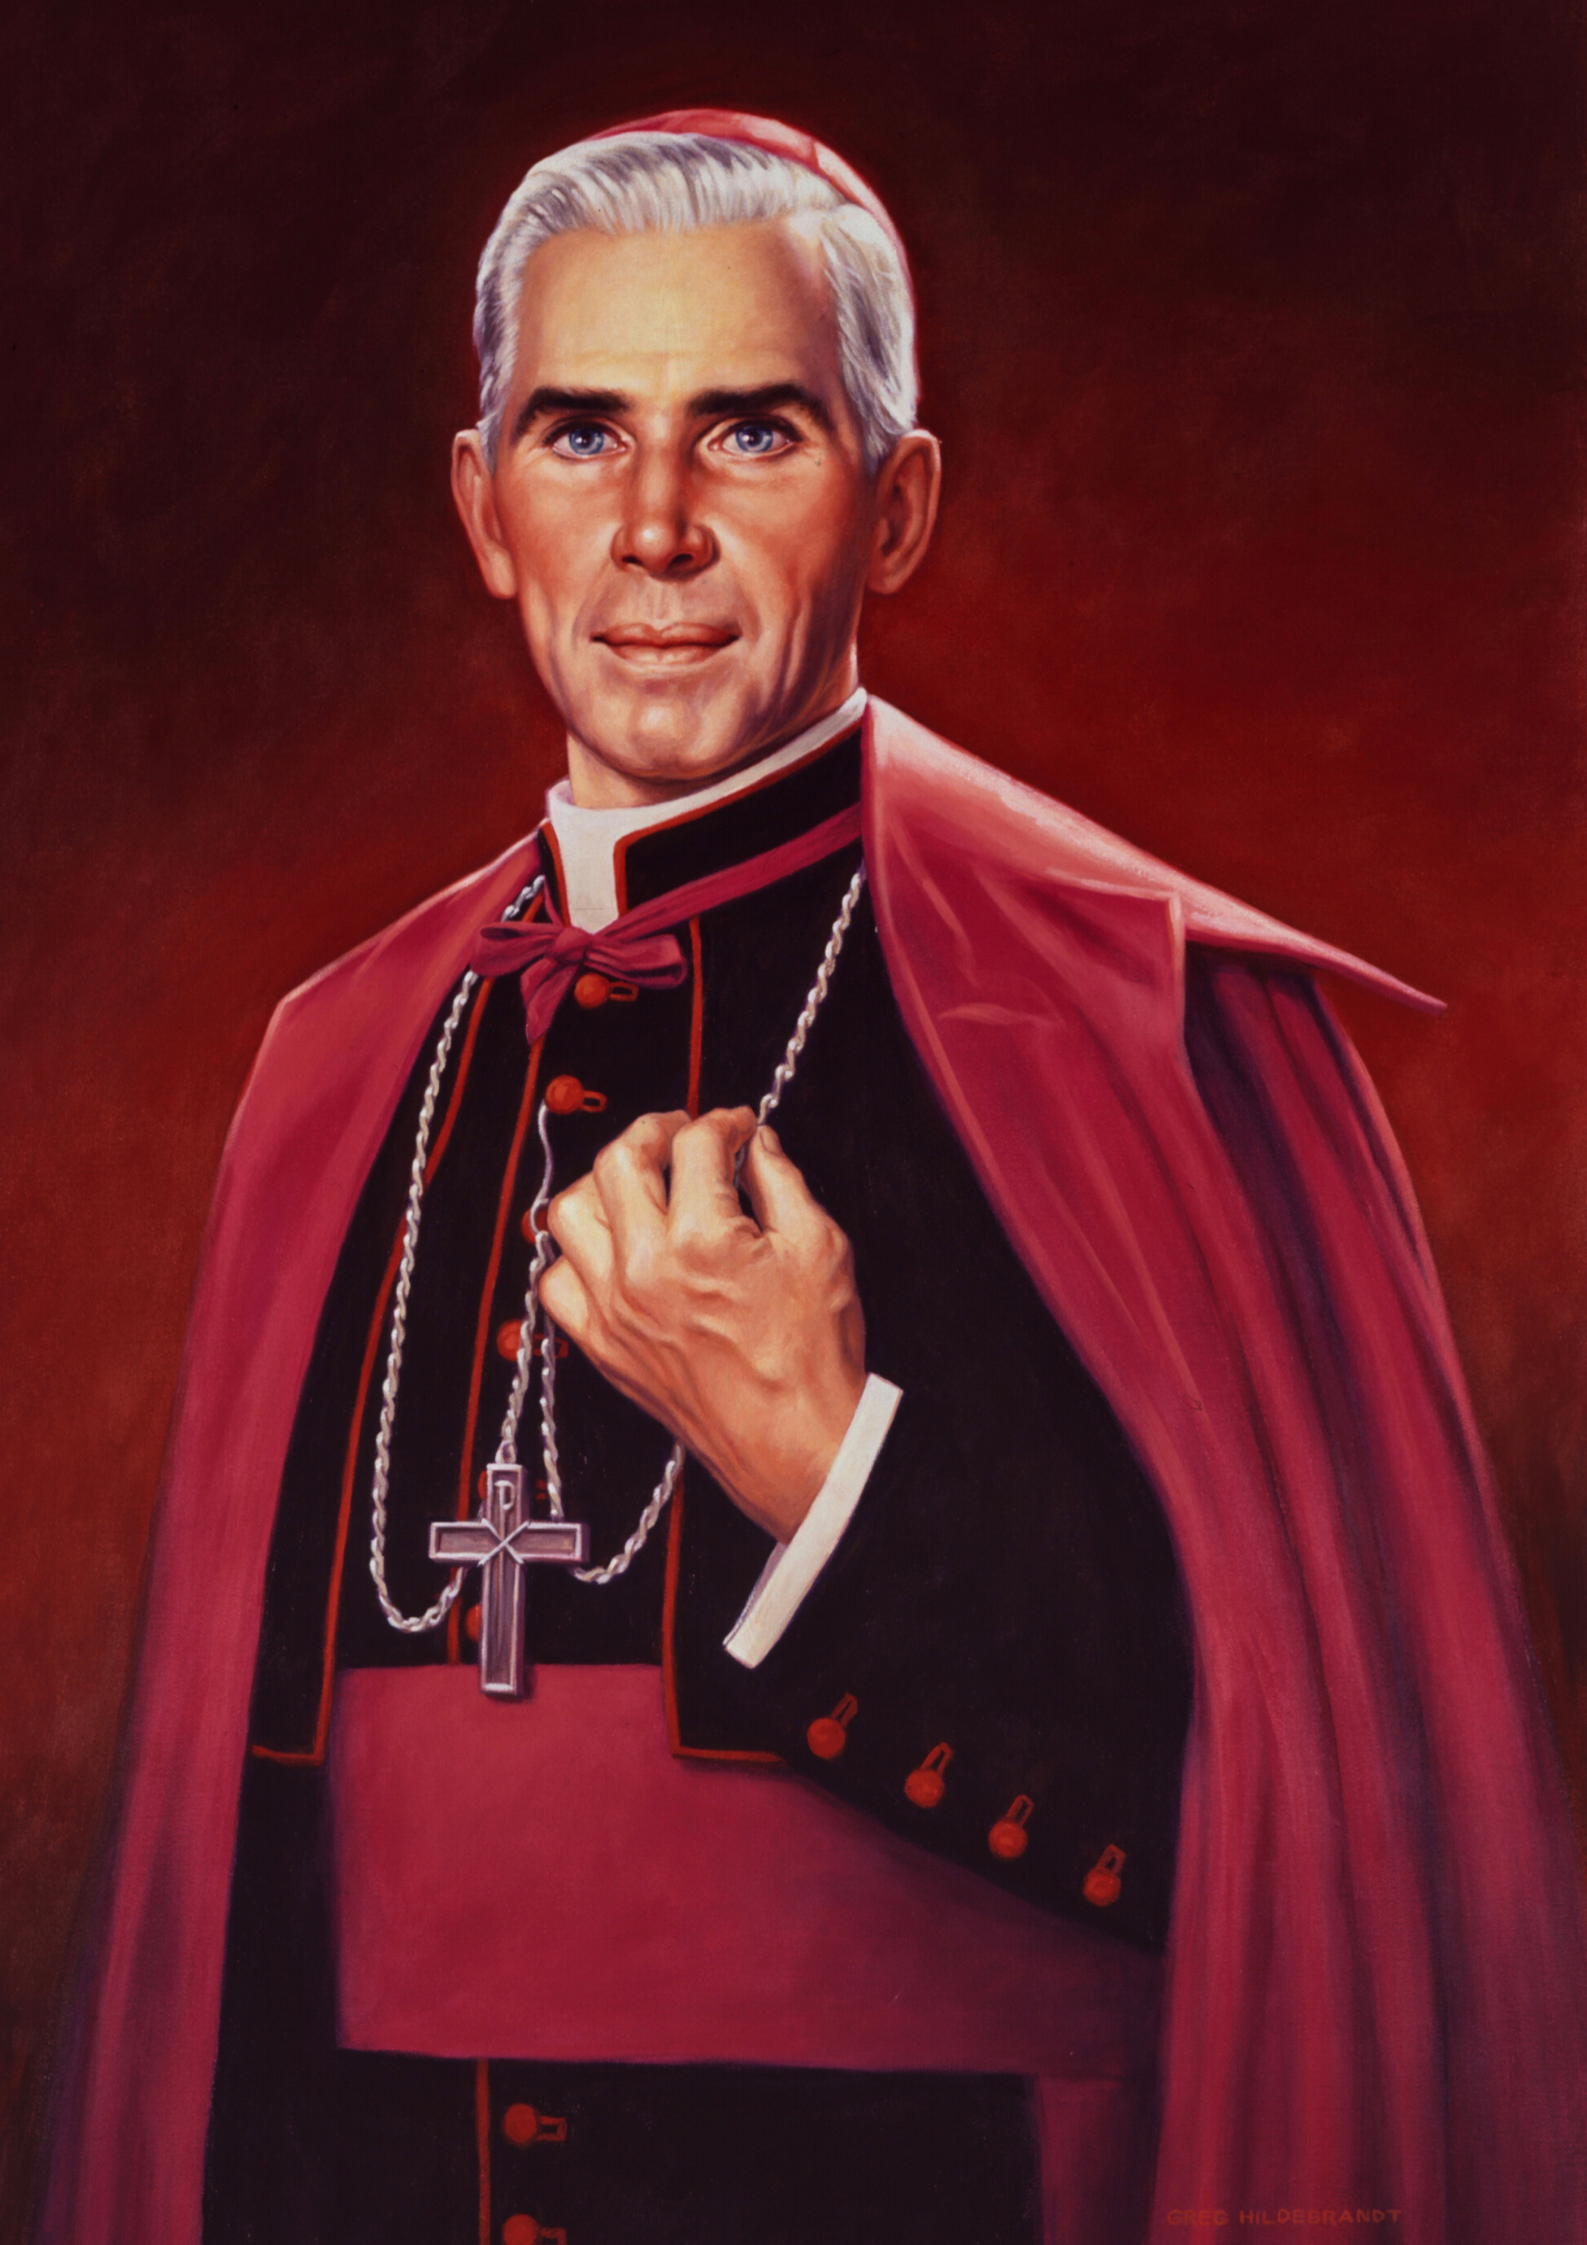
\includegraphics[scale=.8, trim={10cm, 0, 10cm, 0}]{./assets/imagem.jpg}
  \par
   NOVENA A SÃO CLEMENTE MARIA HOFBAUER}
  \date{Início da Novena : 06/03 - Data Litúrgica: 15/03} 
  \author{Garamog, Nina Freitas}


% Comando para fazer "Sumário" não aparecer no Sumário.
\renewcommand{\contentsname}{Sumário}

\begin{document}

\thispagestyle{empty} %zera a primeira página

\maketitle

\newpage
\tableofcontents


\pagestyle{fancy}
\fancyhf{} % clear existing header/footer entries
\fancyfoot[LO, CE]{
\includegraphics[scale=0.2]{./assets/cross.png} São Clemente Maria, rogai por nós! }
% Place Page X of Y on the right-hand
% side of the footer
\fancyfoot[R]{\thepage}

\centering
\vfill
Visite-nos no Telegram: \url{https://t.me/CotidieNovena}

\newpage
%%%%%%%%%%%%%%%%%%%%%%%%%%%%%%%%%%%% História %%%%%%%%%%%%%%%%%%%%%%%%%%%%%%%%%%%%%%%%%%


\begin{justify}
 \section{História}

\begin{justify}
 \subsection{Origens}
\end{justify}
São Clemente Maria Hofbauer nasceu, em 1751, em Tasswitz, na República Tcheca. Seus pais tiveram doze filhos, ele foi o nono filho dessa família muito simples e pobre. Somente recebeu o nome de Clemente quando se tornou eremita. Porém, seu nome de batismo era João.



\begin{justify}
 \subsection{Desde cedo um trabalhador: Padroeiro dos Padeiros}
\end{justify}
Após a morte de seu pai, teve que aprender um ofício. Não tinha condições de continuar os estudos de latim que iniciou na Casa Paroquial até os 14 anos de idade. Foi assim enviado então para uma padaria, em 1770, em um mosteiro. Atuando como padeiro, conheceu duas senhoras em Viena, que se ofereceram para pagar os seus estudos, pois ele não tinha condições para isso.


\vspace{.4cm}
\begin{justify}
 \subsection{Vocação}
\end{justify}

Em 1771, São Clemente Maria Hofbauer viajou a Tivoli para que ali se tornasse eremita, pedindo ao bispo local para assim vestir o hábito. A partir daí, tomou o nome de Clemente Maria. Como eremita, mantinha, em sua vida, a oração e o trabalho sempre muito unidos.

Vivendo pouco tempo como eremita, precisou voltar a seu ofício de padeiro. Com a ajuda das duas distintas senhoras, concluiu os estudos de Filosofia. Não via ser esse o caminho que Deus queria para ele.

Em 1784, Clemente e um amigo fizeram uma peregrinação à Itália e, logo após, decidiram entrar para a vida religiosa. Pouco tempo depois, foram aceitos no noviciado redentorista de São Julião em Roma. No ano seguinte, ele e o amigo professaram seus votos de pobreza, castidade e obediência, no dia de São José em 19 de março. Poucos dias depois, tornou-se sacerdote.


\begin{justify}
 \subsection{São Clemente Maria Hofbauer e o Santo Rosário}
\end{justify}

\begin{justify}
 \subsubsection{Profunda oração}
\end{justify}

Desde criança, sua oração favorita era o Santo Rosário, o qual rezava em família e carregou consigo até o fim de sua vida. Haja vista que também abençoava muitos terços. Dizia sempre que, por esta devoção, conseguia tudo que pedia a Deus, chamando-o de “sua biblioteca”. Nutria assim uma profunda intimidade com Nossa Senhora.

Era uma homem que, literalmente, batia à porta do sacrário. Fazia esta prática nos seus momentos de adoração para que, em seu coração, crescesse uma confiança inabalável em Jesus e sua amizade com ele. Aumentando assim o seu zelo missionário e dizendo para Jesus que estava ali com Ele.

\begin{justify}
 \subsubsection{Seu Apostolado}
\end{justify}

Foi o primeiro redentorista fora da Itália. Mas não podendo exercer sua missão na Áustria, foi enviado para Varsóvia, na Polônia, onde viveu sua missão junto aos pobres órfãos, dando-lhes abrigo e instrução na fé. Assim, o número de rapazes cresceu muito até abrirem o Refúgio Menino Jesus para abrigá-los.


\begin{justify}
 \subsection{A perseguição e o final da vida }
\end{justify}


\begin{justify}
 \subsubsection{Redentoristas}
\end{justify}

Seu apostolado crescia cada vez mais junto aos irmãos redentoristas, criando o que chamavam de Missão perpétua. Ali atendiam confissões a qualquer hora do dia ou da noite, além de realizarem sermões em alemão e polonês todos os dias. Foram perseguidos por todos os lados, tanto na política quanto pelo povo e até na igreja local, chegando a ser impedidos de realizar sermões e atender confissões, a ponto de ficarem presos e, por fim, expulsos do país.

\vspace{.4cm}
\begin{justify}
 \subsubsection{Os últimos dias}
\end{justify}

Voltou para Viena, na Áustria, onde viveu até sua morte no dia 15 de março no ano de 1820. Até o fim da sua vida, atendia os doentes naquele período conturbado de guerras, fazia sermões com enorme sabedoria, e sua fama de santidade crescia evidentemente na cidade, onde, no fim da vida, conseguiu ver a permissão da instalação dos redentoristas na Áustria mesmo com muitas perseguições.

Minha oração
“Jesus, que concedestes a este teu amigo São Clemente Maria, tamanho amor por Ti e zelo missionário, infundi em nossos corações essa mesma disposição para buscar e anunciar o Reino de Deus nesta terra. Dai-nos um profundo desejo pela oração e amor especial pela Santíssima Virgem Maria, para que assim um dia possamos adentrar na Glória Eterna. Amém.”

\href{https://anastpaul.com/2021/03/13/saint-of-the-day-13-march-saint-roderick-died-857-priest-and-martyr/}{\textbf{Créditos: } Anast Paul}

\end{justify}

%%%%%%%%%%%%%%%%%%%%%%%%%%%%%%%%%%%%% Orações %%%%%%%%%%%%%%%%%%%%%%%%%%%%%%%%%%%%%%%%%%%
\begin{justify}

\newpage
\begin{center}
 \section{Orações}\label{sec:Orações} % (fold)
\textit{Em nome do Pai, e do Filho, e do Espírito Santo. Amém.}
\end{center}

Ó Deus misericordioso que, em favor de vosso povo, ornastes São Clemente Maria com um zelo singular pela salvação das almas e por ele anunciastes o Reino de vossa graça, concedei-nos por sua intercessão conservar a fé que ele ensinou e progredir no caminho que ele nos indicou com o exemplo de sua vida. Por ele, concede-nos também a graça de \textit{\textbf{insira o pedido aqui}} Por nosso Senhor Jesus Cristo, vosso Filho, na unidade do Espirito Santo. Amém!

\begin{center}
\textbf{\textit{Pai Nosso, Ave Maria e Glória ao Pai.}}
\end{center}

\vfill

\begin{center}
\section*{São Clemente Maria, Rogai por nós!}
\end{center}

\vfill


\end{justify}

\end{document}
